

\tikzset{every picture/.style={line width=0.75pt}} %set default line width to 0.75pt        

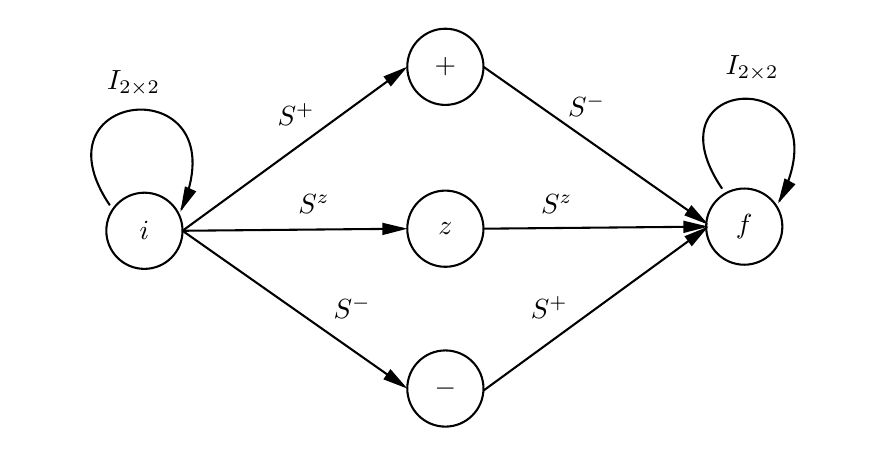
\begin{tikzpicture}[x=0.75pt,y=0.75pt,yscale=-1,xscale=1]
%uncomment if require: \path (0,328); %set diagram left start at 0, and has height of 328

%Shape: Circle [id:dp19428107127030758] 
\draw   (252,96.35) .. controls (252,86.22) and (260.22,78) .. (270.35,78) .. controls (280.49,78) and (288.71,86.22) .. (288.71,96.35) .. controls (288.71,106.49) and (280.49,114.71) .. (270.35,114.71) .. controls (260.22,114.71) and (252,106.49) .. (252,96.35) -- cycle ;

%Shape: Circle [id:dp49492495568136396] 
\draw   (252,174.35) .. controls (252,164.22) and (260.22,156) .. (270.35,156) .. controls (280.49,156) and (288.71,164.22) .. (288.71,174.35) .. controls (288.71,184.49) and (280.49,192.71) .. (270.35,192.71) .. controls (260.22,192.71) and (252,184.49) .. (252,174.35) -- cycle ;
%Shape: Circle [id:dp604607054970826] 
\draw   (252,251.35) .. controls (252,241.22) and (260.22,233) .. (270.35,233) .. controls (280.49,233) and (288.71,241.22) .. (288.71,251.35) .. controls (288.71,261.49) and (280.49,269.71) .. (270.35,269.71) .. controls (260.22,269.71) and (252,261.49) .. (252,251.35) -- cycle ;
%Shape: Circle [id:dp6016992738545592] 
\draw   (107,175.35) .. controls (107,165.22) and (115.22,157) .. (125.35,157) .. controls (135.49,157) and (143.71,165.22) .. (143.71,175.35) .. controls (143.71,185.49) and (135.49,193.71) .. (125.35,193.71) .. controls (115.22,193.71) and (107,185.49) .. (107,175.35) -- cycle ;

%Shape: Circle [id:dp5168816052832117] 
\draw   (396,173.35) .. controls (396,163.22) and (404.22,155) .. (414.35,155) .. controls (424.49,155) and (432.71,163.22) .. (432.71,173.35) .. controls (432.71,183.49) and (424.49,191.71) .. (414.35,191.71) .. controls (404.22,191.71) and (396,183.49) .. (396,173.35) -- cycle ;

%Curve Lines [id:da004973641561244246] 
\draw    (108.71,163.08) .. controls (69.61,105.45) and (172.67,97.16) .. (143.16,165.05) ;
\draw [shift={(142.71,166.08)}, rotate = 294.19] [fill={rgb, 255:red, 0; green, 0; blue, 0 }  ][line width=0.08]  [draw opacity=0] (12,-3) -- (0,0) -- (12,3) -- cycle    ;
%Straight Lines [id:da1995371487826203] 
\draw    (143.71,175.35) -- (250.38,97.53) ;
\draw [shift={(252,96.35)}, rotate = 503.89] [fill={rgb, 255:red, 0; green, 0; blue, 0 }  ][line width=0.08]  [draw opacity=0] (12,-3) -- (0,0) -- (12,3) -- cycle    ;
%Straight Lines [id:da3411444830583379] 
\draw    (143.71,175.35) -- (250.36,250.2) ;
\draw [shift={(252,251.35)}, rotate = 215.06] [fill={rgb, 255:red, 0; green, 0; blue, 0 }  ][line width=0.08]  [draw opacity=0] (12,-3) -- (0,0) -- (12,3) -- cycle    ;
%Straight Lines [id:da19216119538242293] 
\draw    (143.71,175.35) -- (250,174.37) ;
\draw [shift={(252,174.35)}, rotate = 539.47] [fill={rgb, 255:red, 0; green, 0; blue, 0 }  ][line width=0.08]  [draw opacity=0] (12,-3) -- (0,0) -- (12,3) -- cycle    ;
%Straight Lines [id:da07249965960790683] 
\draw    (288.71,174.35) -- (395,173.37) ;
\draw [shift={(397,173.35)}, rotate = 539.47] [fill={rgb, 255:red, 0; green, 0; blue, 0 }  ][line width=0.08]  [draw opacity=0] (12,-3) -- (0,0) -- (12,3) -- cycle    ;
%Straight Lines [id:da2874892398213533] 
\draw    (288.71,96.35) -- (395.36,171.2) ;
\draw [shift={(397,172.35)}, rotate = 215.06] [fill={rgb, 255:red, 0; green, 0; blue, 0 }  ][line width=0.08]  [draw opacity=0] (12,-3) -- (0,0) -- (12,3) -- cycle    ;
%Straight Lines [id:da20880092934159666] 
\draw    (288.71,252.35) -- (395.38,174.53) ;
\draw [shift={(397,173.35)}, rotate = 503.89] [fill={rgb, 255:red, 0; green, 0; blue, 0 }  ][line width=0.08]  [draw opacity=0] (12,-3) -- (0,0) -- (12,3) -- cycle    ;
%Curve Lines [id:da43441994643103965] 
\draw    (403.71,155.08) .. controls (364.61,97.45) and (465.69,95.1) .. (431.24,161.08) ;
\draw [shift={(430.71,162.08)}, rotate = 298.25] [fill={rgb, 255:red, 0; green, 0; blue, 0 }  ][line width=0.08]  [draw opacity=0] (12,-3) -- (0,0) -- (12,3) -- cycle    ;

% Text Node
\draw (270.35,96.35) node    {$+$};
% Text Node
\draw (125.35,175.35) node    {$i$};
% Text Node
\draw (414.35,173.35) node    {$f$};
% Text Node
\draw (120.16,111.78) node [anchor=south] [inner sep=0.75pt]    {$I_{2\times 2}$};
% Text Node
\draw (418.16,104.78) node [anchor=south] [inner sep=0.75pt]    {$I_{2\times 2}$};
% Text Node
\draw (188,112.4) node [anchor=north west][inner sep=0.75pt]    {$S^{+}$};
% Text Node
\draw (310,205.4) node [anchor=north west][inner sep=0.75pt]    {$S^{+}$};
% Text Node
\draw (270.35,174.35) node    {$z$};
% Text Node
\draw (270.35,251.35) node    {$-$};
% Text Node
\draw (328,108.4) node [anchor=north west][inner sep=0.75pt]    {$S^{-}$};
% Text Node
\draw (215,205.4) node [anchor=north west][inner sep=0.75pt]    {$S^{-}$};
% Text Node
\draw (198,156.4) node [anchor=north west][inner sep=0.75pt]    {$S^{z}$};
% Text Node
\draw (315,156.4) node [anchor=north west][inner sep=0.75pt]    {$S^{z}$};


\end{tikzpicture}
